\input{includes/lab_preamble}
\usepackage[utf8]{inputenc}

\def\LabCourse{AP Computer Science A}
\def\LabNumber{07}
\def\LabTitle{Tower of Hanoi Lab}

\begin{document}
	\begin{coverpages}
		\ \\[2cm]
		\begin{center}
			\huge
			\textbf{\LabTitle}

			\Large
			\LabCourse
		\end{center}

		\vspace{1.5cm}

		\begin{center}
			\includegraphics[scale=0.45]{graphics/logo_black}

			\vspace{2.5cm}

			\Large
			Name: \rule{11.5cm}{0.1pt}
		\end{center}
	\end{coverpages}

	\blankpage

	\thispagestyle{empty}
	\tableofcontents

	\pagebreak

	\section{Background}
		In 1883, Édouard Lucas invented a mathematical logic puzzle known as the Tower of Hanoi. In this puzzle, the solver is asked to move a series of different sized disks from one of three pegs, or towers, to another of the pegs. An image of a typical version of this puzzle can be seen below, courtesy of the Wikimedia Commons repository.
		\begin{center}
			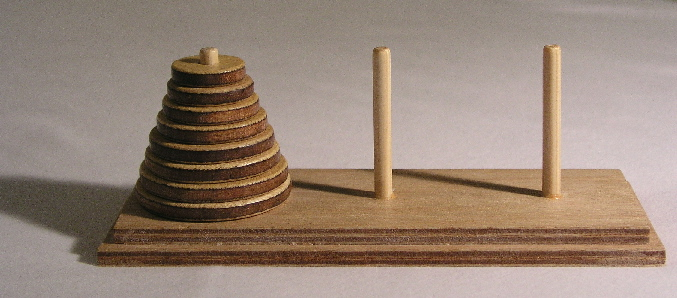
\includegraphics[scale=0.30]{files/Tower_of_Hanoi}

			{\tiny Image by Ævar Arnfjörð Bjarmason, Distributed Under CC Attribution Share-Alike 3.0}
		\end{center}
		Although this might at first seem like a fairly simple task, the following set of rules makes the puzzle far more challenging:
		\begin{enumerate}
			\item Only one disk may be moved at a time.
			\item This disk must be the top disk of one of the pegs/towers.
			\item A larger disk cannot be placed on top of a smaller disk.
		\end{enumerate}

		You are encouraged at this time to actually attempt this puzzle. If a physical copy of the Tower of Hanoi puzzle is not available, there have been multiple adaptations of it online and in mobile apps. A quick search for ``online Tower of Hanoi'' in your favourite search engine or simply ``Tower of Hanoi'' in your app store of choice will turn one up that is free to play. Although the standard puzzle introduced by Lucas had eight disks, you should first try it with fewer disks (I suggest five or fewer). Hopefully, you will not only get a handle on how the rules interact with one another, but also be able to solve the puzzle a few times!

		\subsection{The Minimum Number of Moves}
			Lucas' invention came with a story of the Tower of Brahma. In this story, there exists a temple with three posts and 64 golden disks. According to the myth, Brahmin priests work day and night to transfer the 64 golden disks from one of the posts to the other using the rules above. Once their work is complete, the world will come to an end.\\[\baselineskip]
			Although this stylized version of the Tower of Hanoi puzzle is interesting, the real question that comes out of it is: how long will it take the priests to move these 64 golden disks?\\[\baselineskip]
			It turns out that the answer to the question of the \emph{minimum} number of moves needed to solve the Tower of Hanoi puzzle has been well studied. The minimum number of moves necessary to solve an $n$-disk Tower of Hanoi puzzle is given by the formula:
			\[ 2^{n} - 1 \]
			Note that the derivation of this formula is beyond the scope of this lab; however, it does give us a convenient test to ensure that our algorithms are working efficiently.

			\subsubsection*{Examples}
			\EBox{8-Disk Tower of Hanoi}{Using the formula above, the minimum number of moves required to solve Lucas' original 8-disk puzzle is:
			\[ 2^{8} - 1 = 255 \]}
			\ \\[9pt]
			\EBox{64-Disk Tower of Brahma}{Using the formula above, the minimum number of moves required to solve the Tower of Brahma puzzle is:
			\[ 2^{64} - 1 \approx 1.8 \times 10^{19}\]
			How large is this number? Consider this: if the priests were able to move a single disk every second, twenty-four hours a day, it would take over $584,542,046,090$ \emph{years} for them to complete the puzzle, far exceeding the estimated lifespan of the Universe.
			}

	\pagebreak

	\section{Applications}
		\QBox{Why do you think the Tower of Hanoi puzzle has intrigued computer scientists for decades?}{4cm}
		\ \\[9pt]
		\QBox{Why is it ``natural'' to think of the solution to the Tower of Hanoi puzzle recursively?}{4cm}
		\ \\[9pt]
		\QBox{Using the notation: (source, destination), write every step you need to make to move all disks from the first tower to the third in a three-disk Tower of Hanoi puzzle.\\
			{\small\textbf{Example:} (0, 2) would indicate moving the top disk off the first tower and placing it on the third.}
		}{4cm}
		\ \\[9pt]
		\QBox{Using the same notation as above, now write the steps required to solve a four-disk Tower of Hanoi puzzle; however, this time you also have access to the command: \code{solve3(source, destination)}, which will automatically move the top three disks off of \code{source} and place them on \code{destination}.}{4cm}

	\pagebreak

	\section{Activity \#1}
		\subsection{Introduction}
			In this activity, you will be creating a method that will help you visualize the moves you are making to solve a Tower of Hanoi puzzle, as well as a method used to calculate the tower needed as a ``buffer'' when solving a given puzzle. Although neither of these methods are complex, they will prove to be an immense help in the solving of the actual Tower of Hanoi puzzle in Activity \#2.

		\subsection{Exercises}
		 \begin{enumerate}
		 	\item Implement the \code{performMove()} method. This method should take the following parameters:
				\begin{itemize}[label=>]
					\item \code{puzzle} The Tower of Hanoi puzzle to perform the move on.
					\item \code{from} The source tower to move a disk from.
					\item \code{to} The destination tower to move a disk to.
					\item \code{verbose} Whether or not the move should be output to the screen.
				\end{itemize}
				In particular, you will have to manage the output to the screen. If \code{verbose} is \code{true}, your method should output: \code{Move #} followed by the current move number being performed, as well as a full print out of the current state of the given \code{puzzle}. If the move was unsuccessful, your method should output: \code{Illegal Move} instead. A \code{verbose} value of \code{false} should perform the move silently.\\
				{\small\textbf{Note:} You should use the \code{move()} method built as part of the \code{HanoiPuzzle} class.}

			\item Implement the \code{calcOther()} method. This method should take as parameters the numbers of two towers in the Tower of Hanoi puzzle and return the number of the third, ungiven tower.\\
			{\small\textbf{Note:} Although this can be easily accomplished with a series of \code{if} statements, I encourage you to attempt to find a mathematical formula that can calculate the number of the ungiven tower without a single conditional.}
		 \end{enumerate}

		\subsection{Questions}
			\QBox{Why is it important to be able to ``visually inspect'' each move we make when solving the Tower of Hanoi puzzle?}{4cm}
			\ \\[9pt]
			\QBox{How did you discover the formula for \code{calcOther()}? If you did not discover a formula, still explain the steps you took in your attempts to find one.}{4cm}
	\pagebreak

	\section{Activity \#2}
		\subsection{Introduction}
		\subsection{Exercises}
			\begin{enumerate}
				\item Implement the \code{solve3()} method. This method should take the following parameters:
					\begin{itemize}
						\item \code{puzzle} A 3-disk Tower of Hanoi puzzle to solve.
						\item \code{from} The source tower all of the disks are starting on.
						\item \code{to} The destination tower to move all the disks to.
						\item \code{verbose} Whether or not to output all moves to the screen.
					\end{itemize}
				It will then ``manually'' solve a 3-disk Tower of Hanoi puzzle.\\
				{\small\textbf{Hint:} Use your solution to Question \#3 in the Applications section as a guide.}

				\item Implement the \code{solveN()} method. This method will take the above parameters; however it will also take a parameter, \code{n}, representing how many disks should be moved from the destination tower to the source tower.\\
				{\small\textbf{Hint:} Consider how knowing how to \code{solve3()} helped solving a four-disk puzzle in Question \#4 in the Applications section and implement a recursive solution for \code{solveN()}.}
			\end{enumerate}

		\subsection{Questions}
			\QBox{How did you modify your solution to Question \#3 in the Applications section to account for a potentially variable source and destination tower?}{4cm}
			\ \\[9pt]
			\QBox{Did you use \code{solve3()} in your \code{solveN()} recursion? It turns out that you can use a $1$-disk Tower of Hanoi puzzle as your recursion's base case. Explain how this works.}{4cm}

	\pagebreak

	\section{Final Analysis}
		\QBox{Since its invention, there have been iterative methods developed for solving the Tower of Hanoi puzzle with $n$ disks. Nevertheless, it remains an important academic exercise in the study of recursive algorithms. Why do you think this is?}{4cm}
		\ \\[9pt]
		\QBox{Run the command: \code{solveN(puzzle, 1, 3, 20, true)}. Separately, run: \code{solveN(puzzle, 1, 3, 20, false)}. What do you notice happening? Why do you think this occurs?}{4cm}
		\ \\[9pt]
		\QBox{What challenges did you face in the implementation of \code{solveN()}? How did you overcome these challanges?}{4cm}
		\ \\[9pt]
		\QBox{What new programming techniques or knowledge did you learn as a result of this lab?}{4cm}

	\pagebreak
	\blankpage
	\pagebreak

	\section{Template Class \& Test Cases}
		\lstinputlisting[basicstyle=\small\ttfamily,tabsize=2]{files/TowerOfHanoi.java}

\end{document}
